\chapter{序論}
\label{chap_Introduction}

ハッシュテーブルの挙動を理解する上で,
数理モデルの示す理論的な計算量は大きな助けとなる.
図\ref{fig_taocp_v3_fig44}に\cite{knuth1998}よる比較を示す.
L は linear probing,
U は quadratic probing \footnote{$M \rightarrow \infty$ において,quadratic probing と double hashing は uniform hashing と等価.},
S は separate chaining である.
図\ref{fig_taocp_v3_fig44}が示すように,
load factor が高くなるにつれて,
平均探査回数は上昇する傾向が見られる.
この特性は,
特に linear probing で顕著であるが,
quadratic probing では幾らか改善されている.
しかし,いずれのアルゴリズムも
unsuccessful search では $\alpha = 0.65$ 前後,
successful search でも $\alpha = 0.85$ 前後において,
急激に平均探査回数が増加している
\footnote{
  したがって,性能が悪化する手前でリハッシュし,性能悪化を防ぐことが一般的である.
  なお,リハッシュする load factor は,実装依存である.
}.
一方で,chaining を利用する C, S, SO については,
性能悪化は限られることが分かる.
このとき,
C は coalesced chaining\footnote{Closed hashing の一種で singly linked list により,次に辿る要素を示す.},
S は separate chaining,
SO は separate chaining with ordered lists である.

% Coalesced Chaining
% https://www.youtube.com/watch?v=9SPhD49ePXg
% -> singly linked list (Robin Hood の逆向きの chain.)

% taocp-v3 page.679
% As remarked above, extensive tests show that Algorithm D with two independent
% hash functions behaves essentially like uniform probing, for all practical
% purposes. In fact, double hashing is asymptotically equivalent to uniformprobing, in the limit as M → ∞ (see exercise 70).

% NOTE:   Quadratic Probing and Double Hashing have identical performance.
% Ref: 
%   page. 11
%   DatStr_152_HashTables.pdf - https://www.eecs.yorku.ca/course_archive/2003-04/F/2011/2011A/DatStr_152_HashTables.pdf

\begin{figure} % 特に強い理由がない限り、[htbp]のような指定はしないでください。
  \centering
  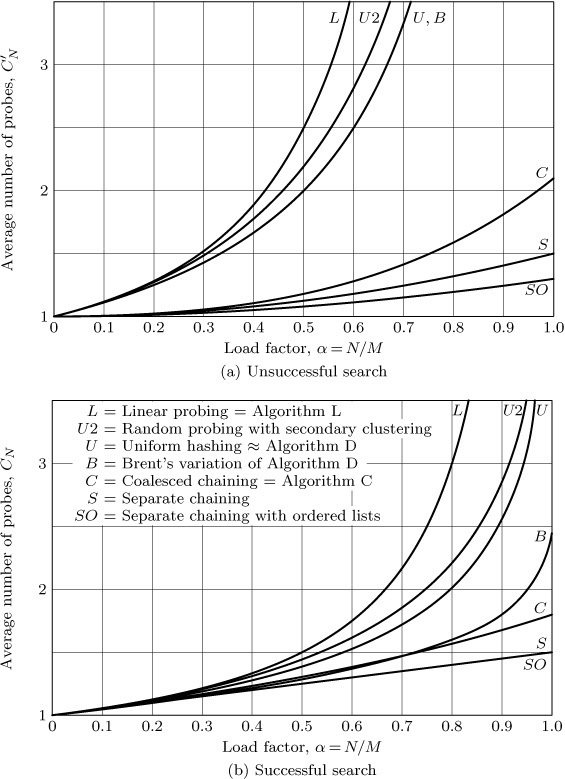
\includegraphics[width=10cm]{./fig/taocp_v3_fig44.png}
  \caption{
    Comparison of collision resolution methods: limiting values of the average number of probes as $M \rightarrow \infty$ \citep{knuth1998}.
    $N$ is a number of elements on the table. $M$ is the table size.
%    N は要素数,M はテーブルサイズを表す.
  }
  \label{fig_taocp_v3_fig44}
\end{figure}

%先行研究\footnote{脚注はこのように挿入します.}.

\section{先行研究}
現実的なハッシュテーブルを検討するには,
単にアルゴリズムのみならず,
対応する実装との比較が望ましい.
ここでは,
実際に利用されているハッシュテーブルの実装を示す.
\leavevmode \newline

{\bf std::unorderd\_map}
\samepage \\ \indent
C++ 標準のハッシュテーブル.
メモリ効率を重視しているため挿入・探査・削除速度は遅い.
アルゴリズムは separate chaining である.
\\

{\bf google::dense\_hash\_map}
\samepage \\ \indent
探査が最も高速な実装の内の 1 つで,\cite{sparsehash2005}に収録されている.
アルゴリズムは quadratic probing である.

ハッシュテーブルが L2 キャッシュに収まるとき,
探査速度は 250 query/$\mu$s 程度 \footnote{AMD Ryzen7 1700 (8C/16T) 3.7 GHz の場合.詳細は,第\ref{chap_Results}章を参照.} であり,
探査 1 回の実行時間は 4 ns
\footnote{
  $
    250{\rm [query \slash \mu s]}
    = \frac{1}{250} {\rm [\mu s \slash query]}
    = \frac{10^3}{250} {\rm [ns \slash query]}
    = 4 {\rm [ns \slash query]}
  $
}
である.このとき,3.7 GHz の CPU では単位クロックあたりの実行時間が,
$2.7 \times 10^{-1}$ [ns/clock]
\footnote{
  $
    \frac{1}{3.7 {\rm [GHz]}}
    = \frac{1}{3.7 \times 10^9}{\rm [sec]}
    = 2.7 \times 10^{-10}{\rm [sec]}
    = 2.7 \times 10^{-1}{\rm [ns/clock]}
  $
}
であるから,1 回の探査で消費する CPU cycle は
15 clock 程度 \footnote
{
  $
    \frac{ 4 {\rm [ns/query]} }{ 2.7 \times 10^{-1} {\rm [ns/clock]} }
    = \frac{ 4 }{ 2.7 \times 10^{-1} } {\rm [clock/query]}
    \simeq 15 {\rm [clock/query]}
  $
} である.

いくつかのハッシュテーブルでは,
キーのハッシュ値をテーブルサイズに丸めるために剰余演算を用いており,
整数除算に必要な CPU cycle は 14\textasciitilde 46 clocks 程度
\footnote{
  \cite{AgnerFog2018}より AMD Ryzen7 1700 の場合.
}
である.
これは,dense\_hash\_map の実行時間に対して計算量が大きい.
実装を確認すると,dense\_hash\_map では整数除算をしておらず,
ハッシュ値の最下位ビット\footnote{英名:Least Significant Bit (LSB).} から
テーブルサイズ分のビット数だけビットマスク演算により取り出している.
これを実現するため,テーブルサイズは常に 2 のべき乗となるように制御されている.

また,キーの 1 つを空マークとして登録する必要があり,キーとして使用できなくなる.
要素の削除が必要な場合は,削除マークも登録する必要があり,同様にキーとして使用できなくなる.
この実装は,メモリ使用量の削減と,それに伴うキャッシュ効率の向上,また,要素探査時のコードの単純化と分岐予測精度の向上が期待される.

Load factor は,探査速度向上のため 50 \% に制限されている.
\\

{\bf ska::flat\_hash\_map}
\samepage \\ \indent
Robin Hood hashing の実装の内の一つ.
条件次第で dense\_hash\_map より探査が高速であることを謳う.
Robin Hood hashing は衝突解決法の一つで,
singly linked list によりハッシュ先のテーブルアドレスを示しており,
次の要素位置を示す coalesced chaining とは singly linked list の使い方が逆である.
本来の挿入位置が分かるため,
要素挿入時に,より近い位置へ要素が移動するよう調整できる.
探査時には,ハッシュ先になるべく近い位置へ移動させられた要素を linear probing により照合する.
Linear probing のコストに配慮し,flat\_hash\_map では
探査を $log_2(n)$ に制限している (ただし $n$ はテーブルサイズ) \citep{Skarupke2017}.

Load factor は,探査速度向上のため 50 \% に制限されている.

\section{研究目的}
理想的なハッシュテーブルは,
衝突がなく,ハッシュ計算の必要もない,単なる配列である.

現実のハッシュテーブルは,
ハッシュを計算し,衝突を解決する必要がある.
また,closed hashing では load factor を 50\textasciitilde 80 \% に制限することが一般的である.
単に高い探査性能を求めるのであれば,
図\ref{fig_taocp_v3_fig44}が示すように load factor を下げてしまえば,
平均探査回数は,どの手法でも同じような回数に落ち着く.
%\footnote{
%  実際に,この味付けが異なるため,ハッシュテーブルの性能を比較する際には,
%  どのハッシュテーブルがどれだけのメモリを消費しているかを考慮しなくてはならず,厳密にな比較は困難である.
%}.
しかし,現実の問題を考えるとき,メモリ資源は有限である.
また,高いメモリ効率を達成すれば,それだけ CPU キャッシュにも乗り易くなる.
加えて,高い load factor まで稼働する程リハッシュしづらく,実利用時の安全マージンも広く取れる.

Open hashing 系のアルゴリズムは chain 構造を持っており,
primary clustering の影響を一切受けない\footnote{性能悪化は secondary clustering によるもの.}.
このため,図\ref{fig_taocp_v3_fig44}に示すように,
closed hashing 系のアルゴリズムよりも平均探査回数が少ない.
一方で,chain 構造はポインタにより実装されるため,
メモリアドレスが不連続となり,キャッシュ効率が悪く,理論上の性能を発揮しない.

Closed hashing 系のアルゴリズムは,
primary clustering による,平均探査回数の悪化が発生し易い.
Primary clustering は特に linear probing で顕著であり,
このため,ska::flat\_hash\_map では探査回数を制限している.
Quadratic probing では primary clustering の影響は小さいものの,
要素を隣接する $1^2, 2^2, 3^2, ... k^2$ 番目の配列に格納するため,
距離が遠い程キャッシュミスし易い.

本研究では,
primary clustering の影響を完全に避けるために chain 構造を採用し,
高いキャッシュ効率を得るために closed hashing を用いる.
このとき,closed hashing に chain 構造を実現するために,
doubly linked list を in-place 実装する.
これにより,従来より高い探査性能を持つハッシュテーブルを実現することが目的である.



